\section{Problem setup}
\label{sec:setup}

% Source: thesis/sections/2_mathematical_background.tex
% \section{Mathematical background}\label{sec:mathematical_background}

\subsection{The forward operator}
\begin{figure}[htbp]
    \centering
    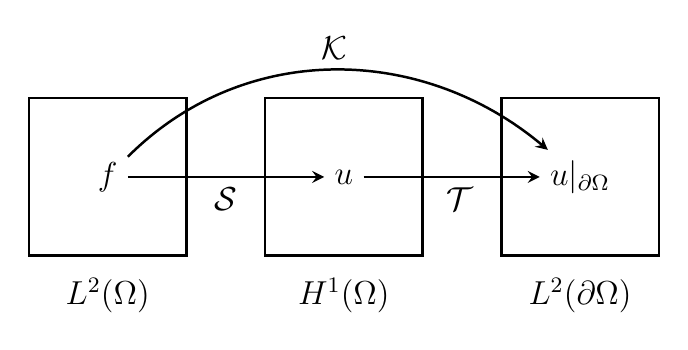
\begin{tikzpicture}[
        >=stealth,
        line width=0.9pt,
        every node/.style={font=\large}
    ]
    % Boxes
    \draw (0,0) rectangle (2,2);
    \draw (3,0) rectangle (5,2);
    \draw (6,0) rectangle (8,2);
    
    % Space labels H^1
    \node at (1,-0.5) {$L^2(\Omega)$};
    \node at (4,-0.5) {$H^1(\Omega)$};
    \node at (7,-0.5) {$L^2(\partial\Omega)$};
    
    % f, u, and u|_dOmega points
    \node (f) at (1,1) {$f$};
    \node (u) at (4,1) {$u$};
    \node (g) at (7,1) {$u|_{\partial\Omega}$};
    
    % Operator S
    \draw[->]
      (f) -- (u)
      node[midway, below, xshift=0.0mm] {$\mathcal S$};
    
    % Operator T
    \draw[->]
      (u) -- (g)
      node[midway, below, xshift=1.0mm] {$\mathcal T$};
    
    % Operator K
    \draw[->]
      (f) to[out=45, in=140]
      node[midway, above] {$\mathcal{K}$}
      (g);
    \end{tikzpicture}
    \caption{The forward operator $\mathcal K = \mathcal T \circ \mathcal S$ maps $f$ to $u|_{\partial\Omega}$.}
    \label{fig:forward_operator}
\end{figure}
Let $\Omega \subset \mathbb R^2$ be a bounded domain with boundary $\partial \Omega$, and consider the boundary value problem (BVP) in Equation~\eqref{eq:pde}. The coefficient $\sigma = \sigma(x) > 0$ denotes the diffusion coefficient and determines the rate and direction of diffusion in the problem. It may be either scalar-valued or matrix-valued. In the latter case, we assume that $\sigma(x)$ is symmetric and positive definite to keep the problem elliptic. The reaction coefficient $c = c(x) > 0$ describes the absorption or decay within the problem. Finally, $f = f(x)$ denotes the source term, which is the unknown input of the inverse problem.

Equation~\eqref{eq:pde} is a linear diffusion-reaction problem with Neumann boundary conditions, and defines a mapping
\begin{equation}\label{eq:S_cont}
    \mathcal S: L^2(\Omega) \rightarrow H^1(\Omega), \quad \mathcal{S} f = u.
\end{equation}
Here, $L^2(\Omega)$ is the space of square integrable functions, and $H^1(\Omega)$ is the Sobolev space of functions in $L^2(\Omega)$ whose weak first derivatives also belong to $L^2(\Omega)$ \cite{quarteroniNumericalModelsDifferential2014}.

To model boundary observations, we introduce the trace operator
\begin{equation}\label{eq:trace}
    \mathcal T: H^1(\Omega) \rightarrow L^2(\partial\Omega), \quad \mathcal{T} u = u|_{\partial\Omega}.
\end{equation}
The term $\mathcal{T} u$ represents the boundary observations of the solution $u$.

The forward operator is then defined as the composition
\begin{equation}\label{eq:K}
    \mathcal K = \mathcal T \circ \mathcal S, \quad \mathcal{K} f = u|_{\partial\Omega},
\end{equation}
which is a mapping from the source function $f$ to the observed output $u|_{\partial\Omega} = \mathcal K f$ on the boundary $\partial \Omega$, see Figure~\ref{fig:forward_operator}.

The associated inverse problem can now be formulated as follows: given boundary data $u|_{\partial\Omega}$, determine a source function $f$ such that
\begin{equation*}
    \mathcal{K} f = u|_{\partial\Omega}.
\end{equation*}
Solving this problem computationally requires discretizing $\mathcal{K}$, understanding the ill-posedness of the resulting system, and regularizing it to obtain stable solutions, which we address in the following sections.


\subsubsection{Ill-posedness}\label{sec:ill_posedness}
A problem is said to be well-posed if its solution exists, is unique, and is stable in the sense that it depends continuously on the data, as formulated by Hadamard \cite{hansen2010discrete}. Denoting $y = u|_{\partial\Omega}$, the inverse problem $\mathcal{K}f = y$ is ill-posed.

The null space of $\mathcal{K}$ is non-trivial: any $f_0$ satisfying $\mathcal{K}f_0 = 0$ can be added to a solution without changing the boundary data $y$. The solution is therefore not unique.

The instability of the solution $f$ is more severe in practice. The compactness of $\mathcal{K}$, and the ellipticity of the PDE in Equation~\eqref{eq:pde}, result in a rapid decay of its singular values towards zero \cite{evansPartialDifferentialEquations2010,engl1996regularization}. Solution components corresponding to small singular values are strongly suppressed by the forward operator and cannot be recovered from noisy data: a small perturbation in $y$ produces a large error in the reconstructed source. This motivates the regularized formulation stated in Equation~\eqref{eq:problem}.


\subsection{Finite element discretization}
\subsubsection{The finite element method}
\begin{figure}[htbp]
    \centering
    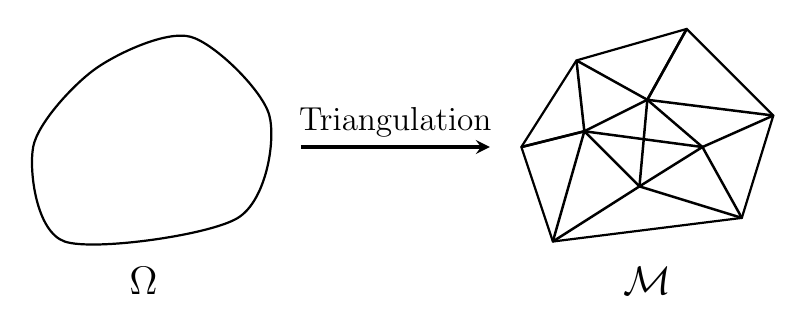
\begin{tikzpicture}[
        >=stealth,
        line width=0.9pt,
        every node/.style={font=\large}
    ]
    % Left: continuous domain Omega
    \begin{scope}[shift={(0,0)}]
      % Draw a smooth-ish domain
      \draw[thick]
        plot [smooth cycle, tension=0.5]
        coordinates {
          (0,0)
          (2.2,0.3)
          (2.6,1.6)
          (1.6,2.6)
          (0.4,2.2)
          (-0.4,1.2)
        };
      % Label
      \node at (1,-0.5) {\Large $\Omega$};
    \end{scope}
    
    % Middle arrow
    \begin{scope}[shift={(4.2,1.2)}]
        \draw[very thick,->] (-1.2,0) -- (1.2,0);
        \node[above] at (0,0) {Triangulation};
    \end{scope}
    
    % Right: triangulated mesh M
    \begin{scope}[shift={(6.2,0)}]
        % Outer polygon (approximation of Omega)
        \coordinate (A) at (0,0);
        \coordinate (B) at (2.4,0.3);
        \coordinate (C) at (2.8,1.6);
        \coordinate (D) at (1.7,2.7);
        \coordinate (E) at (0.3,2.3);
        \coordinate (F) at (-0.4,1.2);
        % Boundary
        \draw[thick] (A)--(B)--(C)--(D)--(E)--(F)--cycle;
        % Some interior points
        \coordinate (P1) at (1.1,0.7);
        \coordinate (P2) at (1.9,1.2);
        \coordinate (P3) at (1.2,1.8);
        \coordinate (P4) at (0.4,1.4);
        % Draw triangulation
        \draw (A)--(P1)--(B);
        \draw (B)--(P2)--(C);
        \draw (C)--(P3)--(D);
        \draw (D)--(P3)--(E);
        \draw (E)--(P4)--(F);
        \draw (F)--(P4)--(A);
        \draw (P1)--(P2)--(P3)--(P4)--cycle;
        \draw (P1)--(P3);
        \draw (P2)--(P4);
        % Label
        \node at (1.2,-0.5) {\Large $\mathcal M$};
    \end{scope}
    \end{tikzpicture}
    \caption{The triangulation $\mathcal{M}$ (the mesh) of $\Omega$. $\mathcal{M}$ is made up of $N$ nodes located at the vertices (corners) of the triangles.}
    \label{fig:triangulation}
\end{figure}
Consider the PDE in Equation~\eqref{eq:pde}. Multiplying the equation by a test function $v \in H^1(\Omega)$, integrating over $\Omega$, and applying Green's identity yields the weak formulation: find $u \in H^1(\Omega)$ such that
\begin{equation}\label{eq:variational_formulation}
    \int_{\Omega} (\sigma \nabla u \cdot \nabla v + c u v) \, dx = \int_{\Omega} f v \, dx,
    \text{ for all } v \in H^1(\Omega).
\end{equation}
For details on the derivation, see Section~4 in Larson and Bengzon \cite{larsonFiniteElementMethod2013}.

Let $\mathcal M$ be a triangulation of $\Omega$ made up of $N$ nodes, with $N_b$ boundary nodes, see Figure~\ref{fig:triangulation} as an example. Introduce the finite element space $V_h \subset H^1(\Omega)$,
\begin{equation}\label{eq:fem_space}
    V_h = \{v \in C^0(\Omega) : v|_M \text{ is linear for all } M \in \mathcal M \}.
\end{equation}
Let $\{\phi_1, \dots, \phi_N\}$ denote a basis for $V_h$, so that
\begin{equation*}
    V_h = \operatorname{span}\{ \phi_1, \dots, \phi_N \}.
\end{equation*}
The basis functions $\phi_i$ are piecewise linear hat functions associated with the nodes of the mesh (see \cite[p.~51]{larsonFiniteElementMethod2013}).

The finite element approximation of \eqref{eq:variational_formulation} then reads: 
find $u_h \in V_h$ such that
 \begin{equation}\label{eq:fem_formulation}
    \int_{\Omega} (\sigma \nabla u_h \cdot \nabla v + c u_h v) \, dx = \int_{\Omega} f v \, dx,
    \text{ for all } v \in V_h.
\end{equation}


\subsubsection{The discrete forward operator}
To obtain a discrete representation of the forward operator 
$\mathcal{K} = \mathcal{T} \circ \mathcal{S}$, 
we discretize both the PDE operator $\mathcal{S}$ and the trace operator $\mathcal{T}$ using the finite element space $V_h$.

Let $f_h, u_h \in V_h$ denote the finite element approximations of $f$ and $u$, respectively. Since $V_h = \operatorname{span}\{\phi_1,\dots,\phi_N\}$, they can be written as
\begin{equation}\label{eq:uh_and_fh}
    f_h = \sum_{j=1}^{N} x_j \phi_j, \quad
    u_h = \sum_{j=1}^{N} u_j \phi_j, 
\end{equation}
with coefficient vectors $x = (x_1,\dots,x_N)^T$, $u = (u_1,\dots,u_N)^T$.

Inserting \eqref{eq:uh_and_fh} into the finite element formulation \eqref{eq:fem_formulation} and testing with the basis functions 
$\{\phi_i\}_{i=1}^N$ yields the linear system
\begin{equation}\label{eq:matrix_system}
    A_h u = M x,
\end{equation}
where $A_h \in \mathbb{R}^{N \times N}$ is the stiffness matrix and $M \in \mathbb{R}^{N \times N}$ the mass matrix, both symmetric positive definite \cite{larsonFiniteElementMethod2013}.
Equation~\eqref{eq:matrix_system} implies that the discrete PDE operator $S$ takes the form
\begin{equation*}
    S = A_h^{-1} M \in \mathbb{R}^{N \times N}.
\end{equation*}
Note that $S$ is a mapping of coefficient vectors: mapping $x$ to $u$.

The trace operator is discretized by a matrix 
$T \in \mathbb{R}^{N_b \times N}$ that extracts the boundary coefficients. If $y$ denotes the vector of boundary coefficients, then
\begin{equation*}
    y = T u.
\end{equation*}

Combining the discrete PDE and trace operators yields the matrix representation of the forward operator,
\begin{equation}\label{eq:discrete_K}
    K = T S = T A_h^{-1} M \in \mathbb{R}^{N_b \times N}.
\end{equation}


\subsubsection{Discrete inner product and norm}
Let $V_h$ be the finite element space introduced in Equation~\eqref{eq:fem_space} and let $f_h, g_h \in V_h$, with coefficient vectors $x, y \in \mathbb{R}^N$, respectively. The $L^2(\Omega)$ inner product of $f_h$ and $g_h$ can be written as
\begin{equation*}
    \langle f_h, g_h \rangle_{L^2(\Omega)} = x^T M y,
\end{equation*}
where $M$ is the mass matrix. 

This induces a discrete inner product on $\mathbb{R}^N$, with associated norm, defined by
\begin{equation}\label{eq:fem_norm}
    \langle x, y \rangle_M = x^T M y,
    \quad
    \| x \|_M = \sqrt{x^T M x}.
\end{equation}

Similarly, let $u, v \in \mathbb{R}^{N_b}$ 
denote coefficient vectors corresponding to the traces 
$u_h|_{\partial\Omega}$ and $v_h|_{\partial\Omega}$. The $L^2(\partial\Omega)$ inner product induces a discrete inner product and norm on $\mathbb{R}^{N_b}$, given by
\begin{equation}\label{eq:fem_norm_ds}
    \langle u, v \rangle_{M_{\partial}}
    = u^T M_{\partial} v,
    \quad
    \| u \|_{M_{\partial}}
    =
    \sqrt{u^T M_{\partial} u},
\end{equation}
where $M_\partial$ denotes the boundary mass matrix.


\subsubsection{The adjoint operator}
Let $\mathcal{K}: L^2(\Omega) \to L^2(\partial\Omega)$ be the bounded linear operator defined in Equation~\eqref{eq:K}. The adjoint operator $\mathcal{K}^*: L^2(\partial\Omega) \to L^2(\Omega)$ is the bounded linear operator satisfying
\begin{equation}\label{eq:K_star_cont}
    \langle \mathcal K f,\, g \rangle_{L^2(\partial\Omega)} =
    \langle f,\, \mathcal K^* g \rangle_{L^2(\Omega)},
\end{equation}
for all $f \in L^2(\Omega)$ and all $g \in L^2(\partial\Omega)$. Such an operator always exists for a bounded linear operator $\mathcal K$ mapping between two Hilbert spaces, see Section~3.9 in Kreyszig for a proof \cite{kreyszigIntroductoryFunctionalAnalysis1989}.

Using the definition in Equation~\eqref{eq:K_star_cont}, we get the weak formulation of $\mathcal{K}^*$ (the adjoint problem): find $w \in H^1(\Omega)$ such that
\begin{equation}\label{eq:variational_formulation_adjoint}
    \int_\Omega (\sigma \nabla w \cdot \nabla v + c w v) \, dx =
    \int_{\partial\Omega} g v \, ds,
    \text{ for all } v \in H^1(\Omega).
\end{equation}
To verify that $\mathcal K^* g = w$, let $u = \mathcal S f$. Testing Equation~\eqref{eq:variational_formulation} with $v = w$ and Equation~\eqref{eq:variational_formulation_adjoint} with $v = u$, and using the symmetry of $\sigma$, gives
\begin{equation*}
    \langle \mathcal K f, g \rangle_{L^2(\partial\Omega)}
    = \int_{\partial\Omega} g u \, ds
    = \int_\Omega f w \, dx
    = \langle f, w \rangle_{L^2(\Omega)}.
\end{equation*}
Thus $w$ satisfies the identity~\eqref{eq:K_star_cont}.

In the discrete case, under the inner products and norms defined in Equations~\eqref{eq:fem_norm} and~\eqref{eq:fem_norm_ds}, the adjoint operator $K^* \in \mathbb{R}^{N \times N_b}$ of $K \in \mathbb{R}^{N_b \times N}$ satisfies
\begin{equation}\label{eq:K_star_def}
    (K x)^T M_\partial y = x^T M K^* y,
\end{equation}
for all $x \in \mathbb R^N$ and all $y \in \mathbb R^{N_b}$.

Inserting the explicit representation of $K$ given in Equation~\eqref{eq:discrete_K} and using the symmetry of $A_h$ yields the matrix representation of $K^*$,
\begin{equation}\label{eq:discrete_K_star}
    K^* = A_h^{-1} T^T M_\partial,
\end{equation}
where $A_h$ is the stiffness matrix, $T$ the discrete trace operator, and $M_\partial$ the boundary mass matrix.


\subsection{Tikhonov regularization}
Let $A \in \mathbb{R}^{m \times n}$ and consider the inverse problem $Ax = y$. If $A$ is ill-conditioned, the matrix $A^T A$ in the normal equations $A^T A x = A^T y$ is also ill-conditioned, and small perturbations in $y$ 
cause large changes in the solution. Tikhonov regularization stabilizes the problem by solving
\begin{equation}\label{eq:tikhonov}
    \min_{x \in \mathbb{R}^n}
    \|Ax - y\|^2 + \lambda^2 \|Wx\|^2,
\end{equation}
where $\lambda \ge 0$ is the regularization parameter and $W \in \mathbb{R}^{n \times n}$ is the weight matrix. The normal equations of Equation~\eqref{eq:tikhonov} are $(A^T A + \lambda^2 W^T W) x = A^T y$, so if $W$ is diagonal with $\operatorname{diag}(W) > 0$ and $\lambda > 0$, then $(A^T A + \lambda^2 W^T W)$ is SPD, stabilizing the problem and making the solution unique.

The weights $W$ can include prior knowledge about the solution to penalize specific types of unwanted solutions \cite{hansen2010discrete}. With $W = I$, this is standard Tikhonov regularization.


\subsection{SVD and low-rank approximations}
The rapid decay of the singular values of $K$ makes it possible to approximate $K$ well by a low-rank matrix. Its right singular vectors also determine the regularization weights in Section~\ref{sec:the_discrete_inverse_problem}.

\subsubsection{Singular value decomposition}\label{sec:svd}
The singular value decomposition of a matrix $A\in\mathbb R^{m\times n}$ of rank $q$ is $A=U\Sigma V^T$, where $U\in\mathbb R^{m\times q}$ and $V\in\mathbb R^{n\times q}$ have orthonormal columns and $\Sigma=\operatorname{diag}(\sigma_1,\dots,\sigma_q)$ with $\sigma_1\ge\cdots\ge\sigma_q>0$. The columns $u_i$ and $v_i$ of $U$ and $V$ are the left and right singular vectors of $A$, respectively.

Keeping the first $k$ singular values and the corresponding singular vectors gives the truncated SVD (tSVD),
\begin{equation}\label{eq:tsvd}
    A_k = U_k\Sigma_k V_k^T.
\end{equation}
By the Eckart--Young--Mirsky theorem \cite{eckartApproximationOneMatrix1936}, $A_k$ is the best approximation of $A$, with its error in the spectral norm satisfying
\begin{equation}\label{eq:svd_error}
    \|A-A_k\|_2 = \min_{\operatorname{rank}(X)\le k}\|A-X\|_2 = \sigma_{k+1}.
\end{equation}
Truncating small singular values regularizes the pseudoinverse \cite{hansen2010discrete}. The tSVD also provides a reference for the randomized approximation of $K$ in Section~\ref{sec:rsvd}.


The Moore--Penrose pseudoinverse of $A$ is
\begin{equation}\label{eq:pseudoinverse}
    A^+ = V\Sigma^{-1}U^T,
\end{equation}
where $\Sigma^{-1}=\operatorname{diag}(1/\sigma_1,\dots,1/\sigma_q)$. For the least-squares problem $\min_x\|Ax-y\|_2$, $A^+y$ is the solution with the smallest Euclidean norm \cite[Section~5.5]{golubMatrixComputations4th2013}. The identity $A^+A=VV^T$ gives the orthogonal projection onto the row space of $A$, used below to compute the regularization weights.

For a nonsingular square matrix $A\in\mathbb R^{n\times n}$, the condition number in the spectral norm is $\kappa(A)=\sigma_1/\sigma_n$ \cite{hansen2010discrete}.


\subsubsection{Randomized SVD}
The randomized SVD is a technique used to compute a rank-$k$ approximation of an $m\times n$ matrix without computing the SVD. The core idea is to use random sampling $Y = A \Psi$ with a random matrix $\Psi$ to find a low-rank matrix $Q = \operatorname{orth}(Y)$ which approximates the range of $A$, project $A$ onto $\operatorname{range}(Q)$, and compute the SVD of the projection. The projection $QQ^T A$ will, with high probability, capture the dominant actions of $A$ \cite{halkoFindingStructureRandomness2011}. Computing $B = Q^T A$ and its SVD $B = \tilde U \Sigma V^T$ then gives an approximate SVD $A \approx (Q \tilde U) \Sigma V^T$. This procedure is summarized in Algorithm \ref{alg:rsvd}. The basis $Q$ is obtained via a QR factorization of $Y$.

Let $A_k$ denote a rank-$k$ approximation of $A$ obtained using rSVD with a random test matrix $\Psi$. Error analysis of rSVD is an active area of research. Halko et al. derived initial reference error analysis in terms of expectation \cite{halkoFindingStructureRandomness2011}, which was later improved upon by Gu \cite{guSubspaceIterationRandomization2015}. Diouane et al. have recently derived further improvements \cite{diouaneGeneralErrorAnalysis2022}.

Although theoretical upper bounds are useful in many applications, it is well known that randomized algorithms for low-rank approximations, like Algorithm~\ref{alg:rsvd} and the like, far outperform their error bounds in numerical experiments \cite{halkoFindingStructureRandomness2011,guSubspaceIterationRandomization2015,rokhlinFastRandomizedAlgorithm2008}.
\begin{algorithm}[!htbp]
\caption{rSVD}
\label{alg:rsvd}
\begin{algorithmic}[1]
    \Require $A\in\mathbb R^{m\times n}$, target rank $k$, oversampling parameter $p$
    \Ensure Approximate rank-$k$ factorization $U\Sigma V^T$
    \State Generate a random $n\times(k+p)$ test matrix $\Psi$
    \State Compute $Y = A\Psi$
    \State Form an orthonormal basis $Q$ of $Y$
    \State Set $B = Q^TA$
    \State Compute the SVD $B = \tilde U\Sigma V^T$
    \State Set $U = Q\tilde U$
    \State Truncate to rank $k$: $U, \Sigma, V^T \leftarrow \operatorname{truncate}_k(U, \Sigma, V^T)$
\end{algorithmic}
\end{algorithm}


\subsection{The discrete inverse problem}\label{sec:the_discrete_inverse_problem}
\begin{figure*}[thbp]
    \centerline{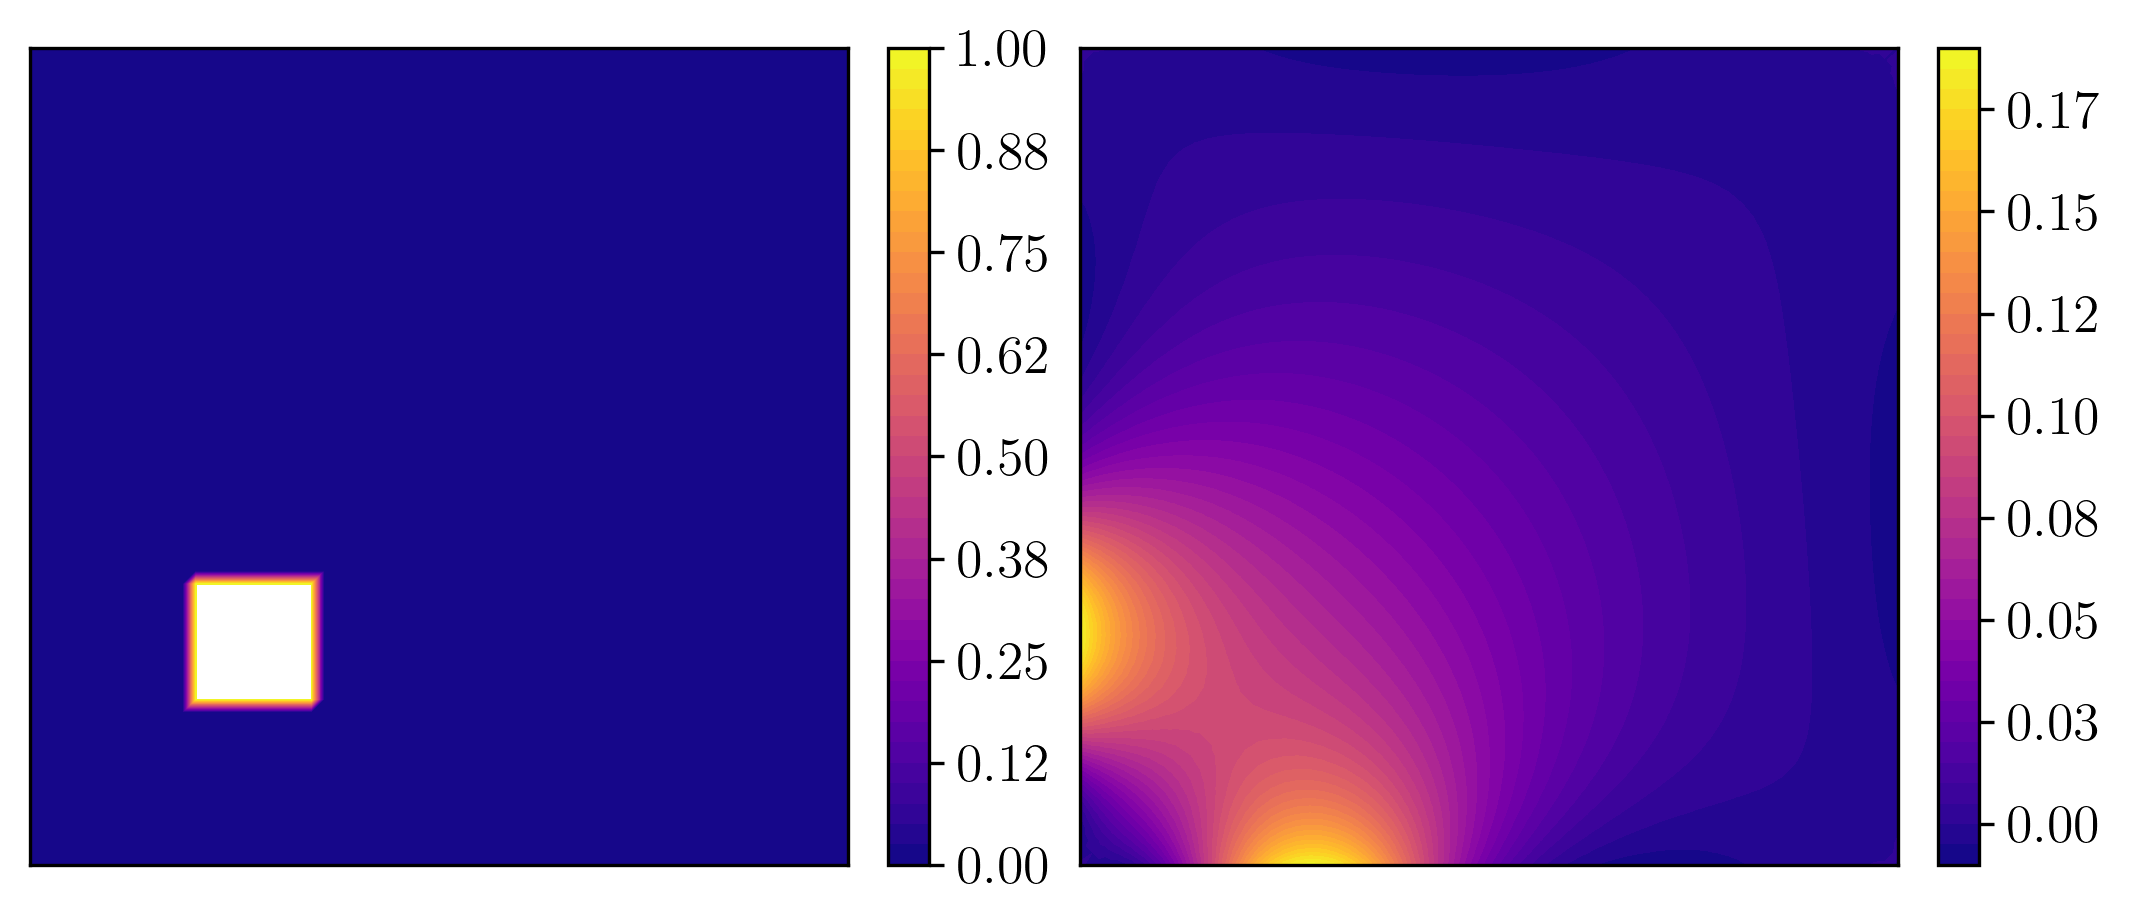
\includegraphics[width=0.75\textwidth]{standard_tikhonov_solution.png}}
    \caption{The true source $x$ (left) and a standard Tikhonov solution $x_\lambda$ (right), where $\lambda = 10^{-4}$.}
    \label{fig:standard_tikhonov_solution}
\end{figure*}
Replacing $\mathcal{K}$ by its discretization $K \in \mathbb{R}^{N_b \times N}$ and the $L^2$ norms by the FEM inner products in Equations~\eqref{eq:fem_norm} and~\eqref{eq:fem_norm_ds}, the Tikhonov problem in Equation~\eqref{eq:problem} takes the discrete form
\begin{equation}\label{eq:discrete_inverse_problem}
    \min_{x \in \mathbb{R}^N}
    \| K x - y \|_{M_\partial}^2
    + \lambda^2 \| W x \|_M^2,
\end{equation}
where $x \in \mathbb{R}^N$ is the coefficient vector of $f_h \in V_h$, $y \in \mathbb{R}^{N_b}$ is the observed boundary data, $\lambda \ge 0$ is the regularization parameter, and $W$ the regularization weight matrix.

Standard Tikhonov ($W = I$) does not work here. Because $K$ has a large null space, the solutions it produces concentrate near the domain boundary regardless of where the true source is located \cite{elvetunRegularizationOperatorSource2020}. This is illustrated in Figure~\ref{fig:standard_tikhonov_solution}.


\subsubsection{Regularization weights}
Assume that $\{ \phi_i \}$ is an orthonormal basis of $V_h$, let $\operatorname{Nul}(\mathcal{K})$ denote the null space of $\mathcal{K}$ and $\operatorname{Nul}(\mathcal{K})^\perp$ its orthogonal complement. Any source $f \in V_h$ can be written as $f = f_\perp + f_0$, where $f_\perp \in \operatorname{Nul}(\mathcal{K})^\perp$ and $f_0 \in \operatorname{Nul}(\mathcal{K})$. As Elvetun and Nielsen point out in \cite{elvetunRegularizationOperatorSource2020}, sources $f$ located near the domain boundary have a larger $f_\perp$ component, and sources deep within the domain have a larger $f_0$ component. If $f^* = \mathcal{K}^+ y$ denotes the least-squares minimum-norm solution, they show that for the case when $f = \phi_j$, we have that
\begin{equation*}
    f^* = \sum_{i} \langle \hat P f, \phi_i \rangle \phi_i,    
\end{equation*}
where $\hat P: V_h \to \operatorname{Nul}(\mathcal{K})^\perp$ is the orthogonal projection onto $\operatorname{Nul}(\mathcal{K})^\perp$. Since $\hat{P}\phi_i = \phi_{i,\perp}$, basis functions deep in the interior have small $\|\hat{P}\phi_i \|$. By the Cauchy-Schwarz inequality, if $\| \hat P \phi_i \|$ is small, then $\langle \hat Pf, \phi_i \rangle$ is small, and the corresponding component of $f^*$ is small. This means that for any $\phi_i$ far away from $\partial \Omega$, the corresponding component of $f^*$ is forced to be small, introducing bias to the solution. This issue transfers to the standard Tikhonov solution $f_\lambda$ since $f_\lambda \to f^*$ as $\lambda \to 0$ \cite{engl1996regularization}.

Elvetun and Nielsen counteract this by re-scaling the norm of $\hat P \phi_i$ such that $\| \hat P \phi_i \| = 1$. This is achieved by setting $w_i = \| \hat P \phi_i \|$ with $W = \operatorname{diag}(w_i)$ in the Tikhonov formulation, equalizing the contribution of all components. In the discrete formulation, $\hat P = K^+ K$ is the orthogonal projection onto the complement of the null space, and the weights are computed as $w_i = \|K^+ K e_i\|$.

In our setting, the basis of the element space $V_h$ given in Equation~\eqref{eq:fem_space} needs to be normalized to match the orthonormality assumption made above. If $K = U\Sigma V^T$ is the SVD of $K$ and $M_{ii}$ is the $i$-th diagonal element of the mass matrix $M$, then the weights are computed as 
\begin{equation}\label{eq:weights}
    w_i =
    \frac{\| K^+ K e_i \|_M}
         {\| \phi_i \|_M} =
    \frac{\| V V^T e_i \|_M}
         {\sqrt{M_{ii}}},
    \quad i = 1, \dots, N,
\end{equation}
and $W = \operatorname{diag}(w_1, \dots, w_N)$.


\subsubsection{A transformed formulation}
The weights in Equation~\eqref{eq:weights} are defined by measuring length in the subspace $\operatorname{Nul}(K)^\perp \subset \mathbb{R}^N$. However, the residual vector $K x - y$ in Equation \eqref{eq:discrete_inverse_problem} is measured in the boundary space $\mathbb{R}^{N_b}$. Following Elvetun and Nielsen in \cite{elvetunWeightedSparsityRegularization2023}, we can reformulate the equation $K x = y$ as the equivalent problem $K^+ K x = K^+ y$ (since $K$ and $K^+K$ share the same nullspace). Now, the residual $K^+ K x - K^+ y$ lives in the subspace $\operatorname{Nul}(K)^\perp$, the same space where the weights $w_i$ are defined. Motivated by this, we replace the original residual by the transformed one, giving
\begin{equation}\label{eq:transformed_discrete_inverse_problem}
    \min_{x \in \mathbb{R}^N}
    \| K^+ K x - K^+ y \|_{M}^2
    + \lambda^2 \| W x \|_M^2.
\end{equation}

In practice, the pseudoinverse $K^+$ amplifies errors associated with small singular values of $K$, and must therefore be approximated by the truncated pseudoinverse $K_k^+$, obtained by keeping the first $k$ singular components in Equation~\eqref{eq:pseudoinverse}. The weights are correspondingly approximated using $P_k = K_k^+ K$.
